\section{Solare Strahlung}


\subsection{Air Mass (AM)}

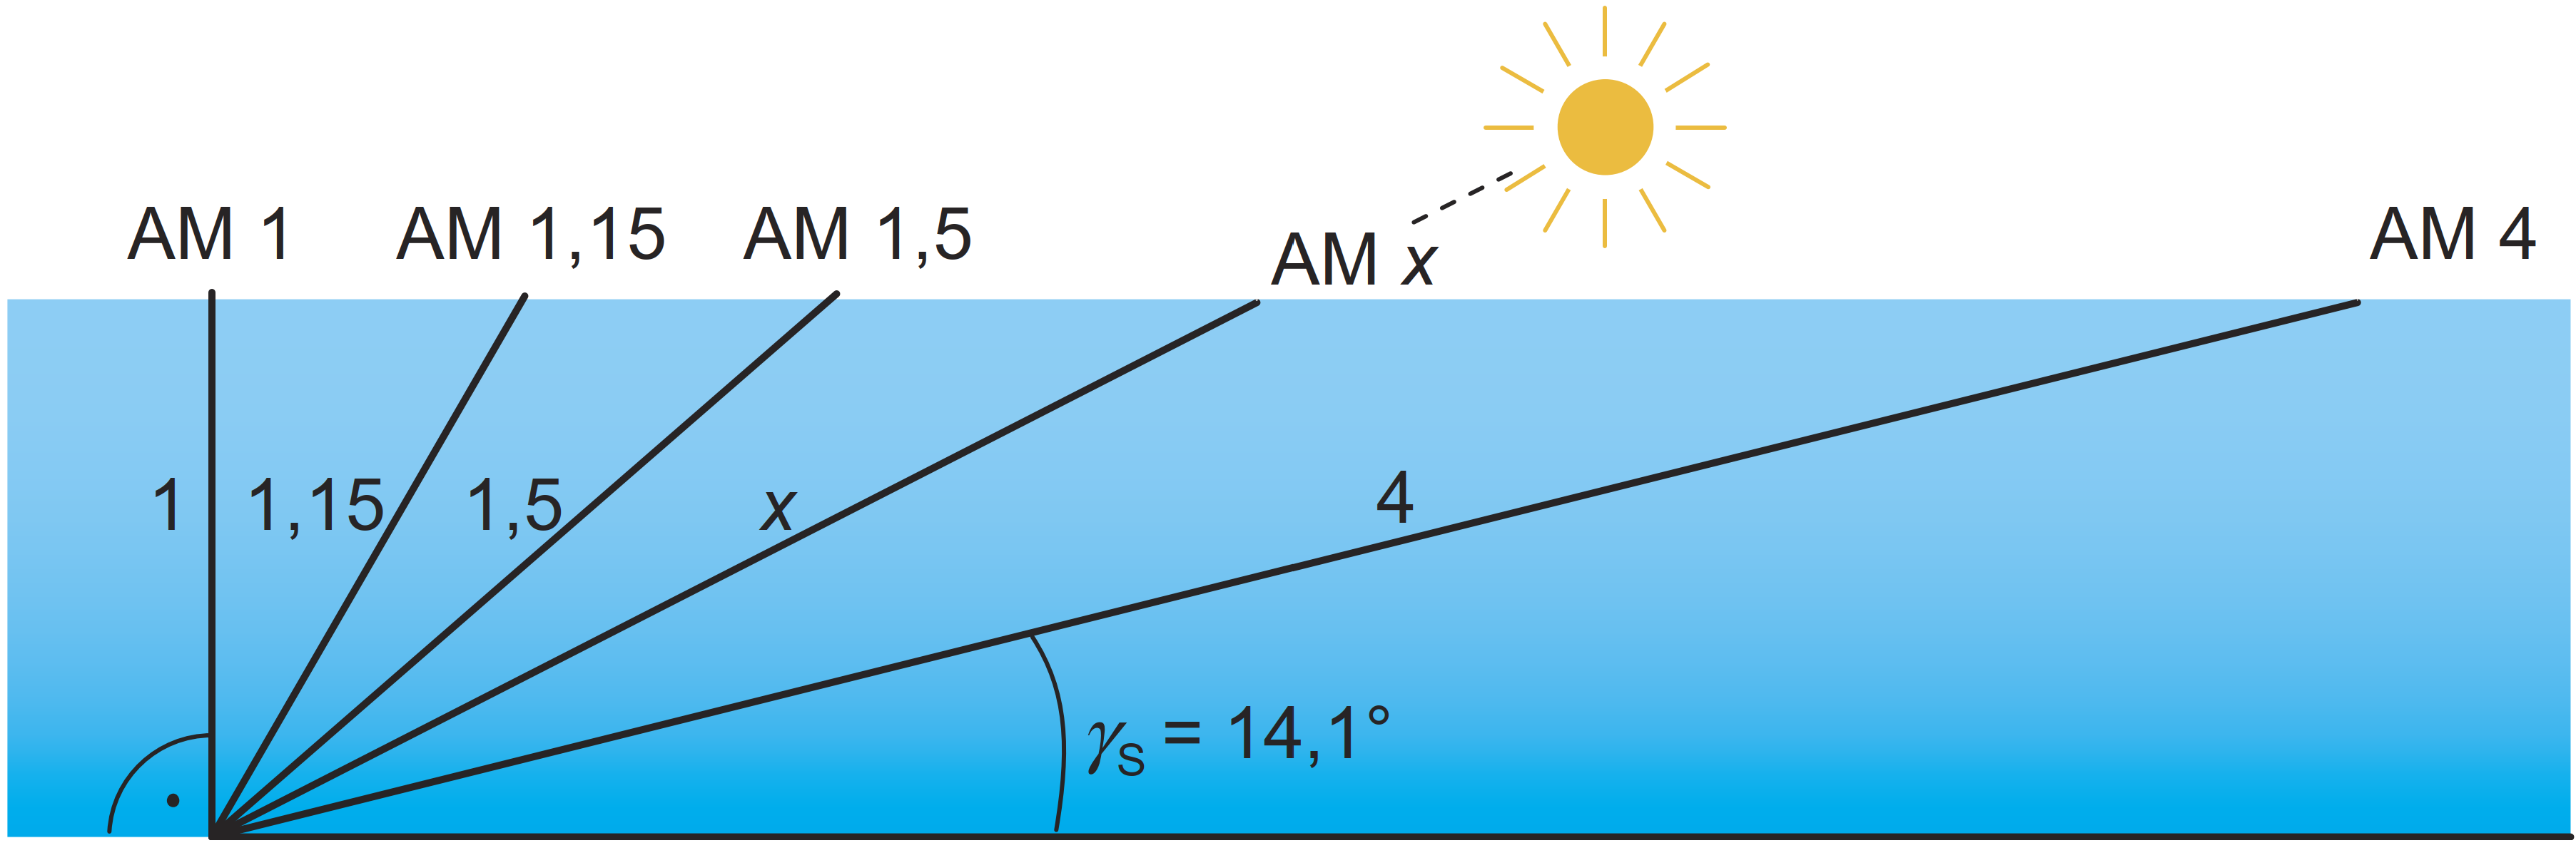
\includegraphics[width=0.95\columnwidth]{images/V01_01.png}

$\boxed{x = \frac{1}{\sin(\gamma_s)}}$

\renewcommand{\arraystretch}{1} % Erhöht Zeilenhöhe für bessere Lesbarkeit
\begin{tabular}{@{} l p {4cm} l @{}}
    [$x$]           & Air Mass Wert         \dotfill & 1            \\
    $[\gamma_{s}]$  & Sonnenstandswinkel    \dotfill & $^\circ$     \\ 
\end{tabular}

\subsection{Solar Spektrum}
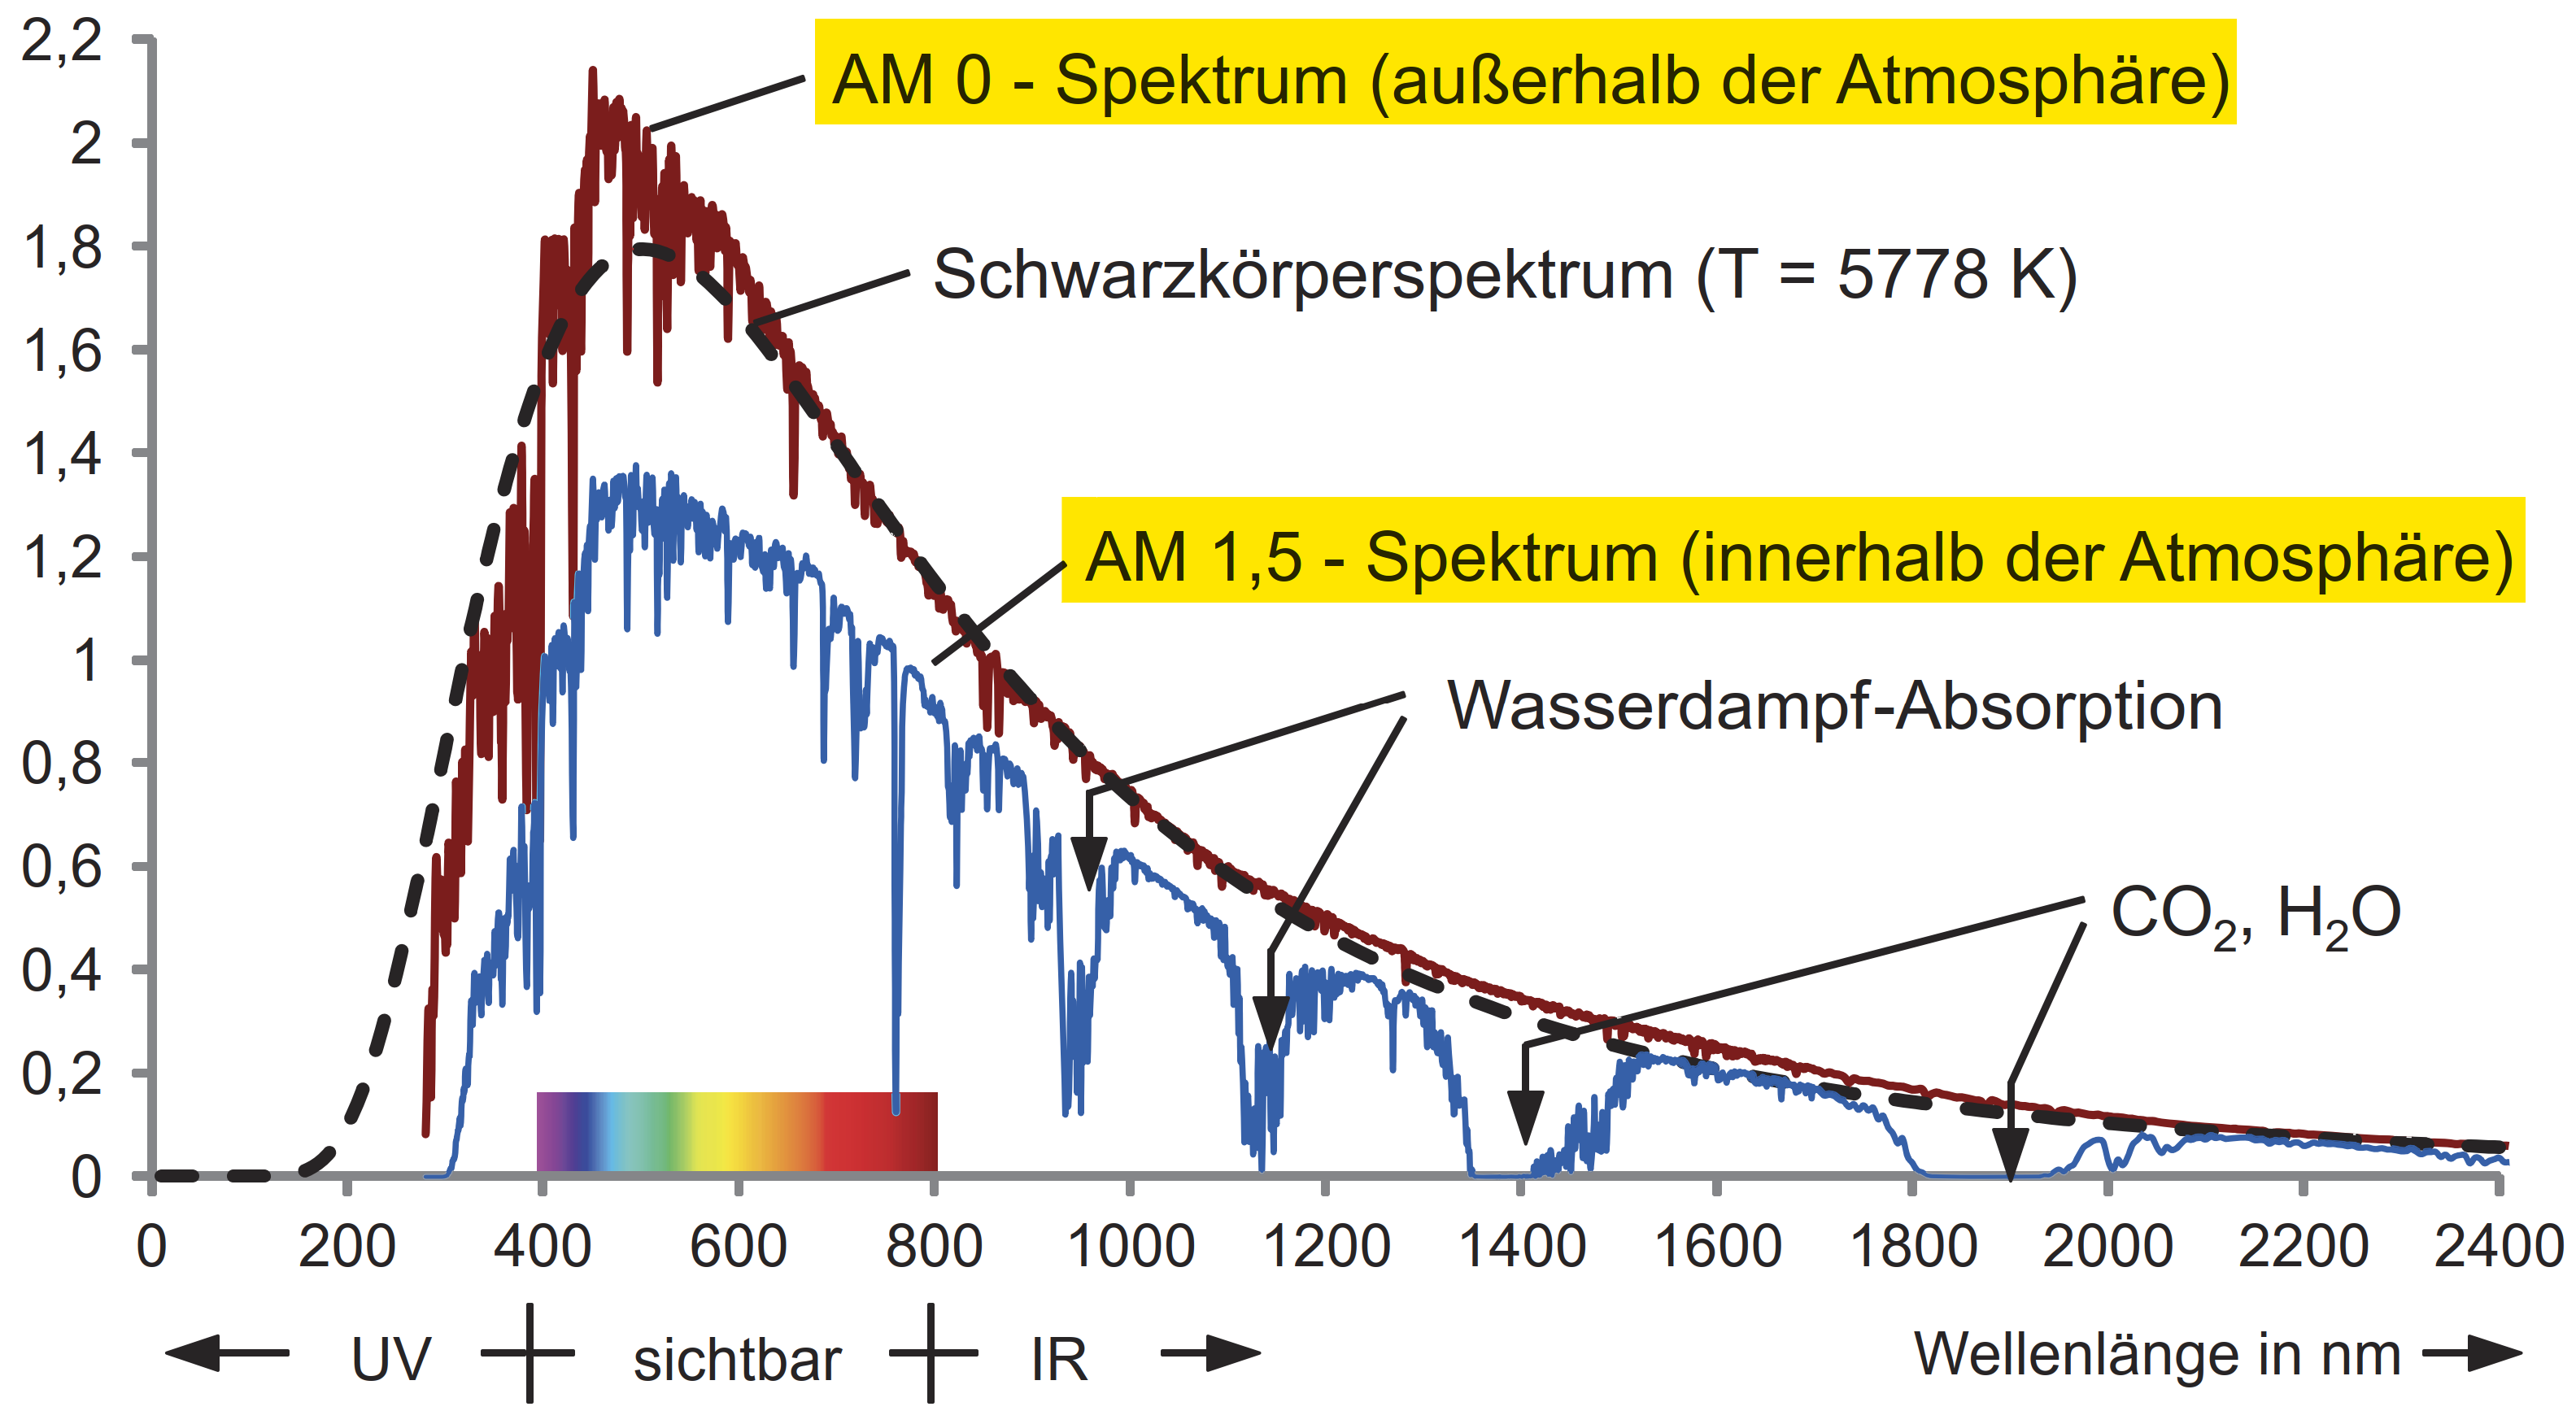
\includegraphics[width=0.95\columnwidth]{images/V01_01.1.png}\\

\renewcommand{\arraystretch}{1.2} % Erhöht Zeilenhöhe für bessere Lesbarkeit
\begin{tabular}{@{} l p {4cm} l @{}}
    $[E_{e,\lambda}]$   & Spektrake Bestrahlungsstärke  \dotfill & $\frac{\watt}{\meter^2 \cdot \text{n} \meter}$ \\
    $[E_{S}]$           & Solarkonstante                \dotfill & $\frac{\watt}{\meter^2}$ \\
    $[\lambda]$         & Wellenlänge                   \dotfill & $\text{n} \meter$ \\ 
\end{tabular}

\subsubsection{Berechnung der Solarkonstante $E_S$}
$E_S = \frac{\text{Strahlungsleistung}}{\text{Kugeloberfläche}}
= \frac{P_{\text{Sonne}}}{4 \cdot \pi \cdot r_{\text{SE}}^2}
= \frac{3{,}845 \cdot 10^{26} \text{ W}}{4 \cdot \pi \cdot (1{,}496 \cdot 10^{11} \text{m})^2}
= 1361 \, \frac{\text{W}}{\text{m}^2}$

\subsection{Global-, Direkt- und Diffusstrahlung}
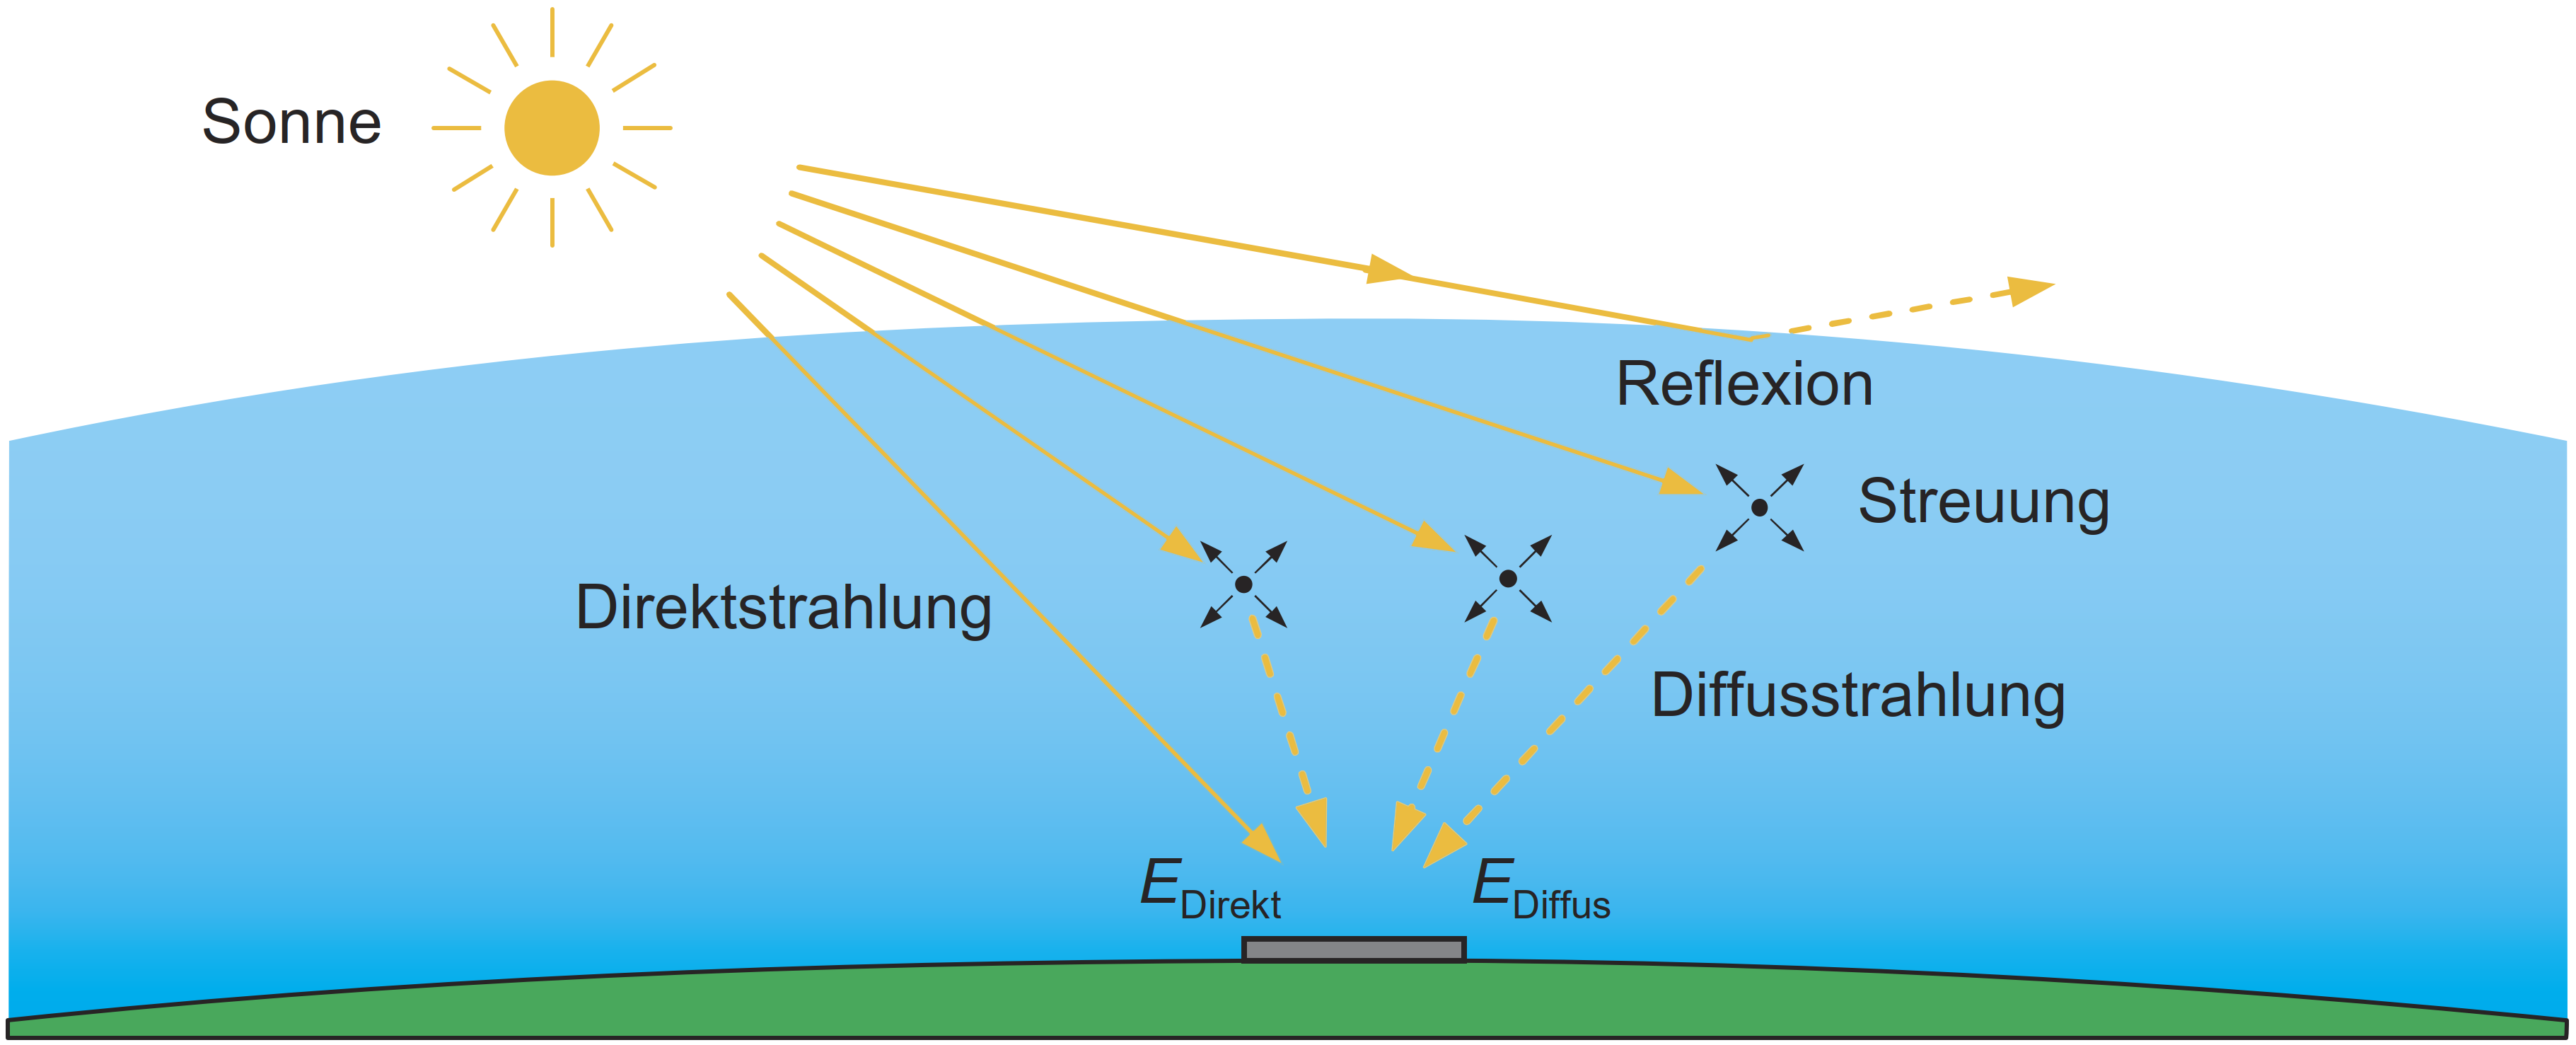
\includegraphics[width=0.95\columnwidth]{images/V01_02.png}

$\boxed{E_G = E_{Dir} + E_{Diff}}$

\renewcommand{\arraystretch}{1.2} % Erhöht Zeilenhöhe für bessere Lesbarkeit
\begin{tabular}{@{} l p {4cm} l @{}}
    $[E_{G}]$       & Globalstrahlung  \dotfill & $\frac{\watt}{\meter^2}$ \\
    $[E_{Dir}]$     & Direktstrahlug   \dotfill & $\frac{\watt}{\meter^2}$ \\
    $[E_{Diff}]$    & Diffusstrahlung  \dotfill & $\frac{\watt}{\meter^2}$ \\ 
\end{tabular}

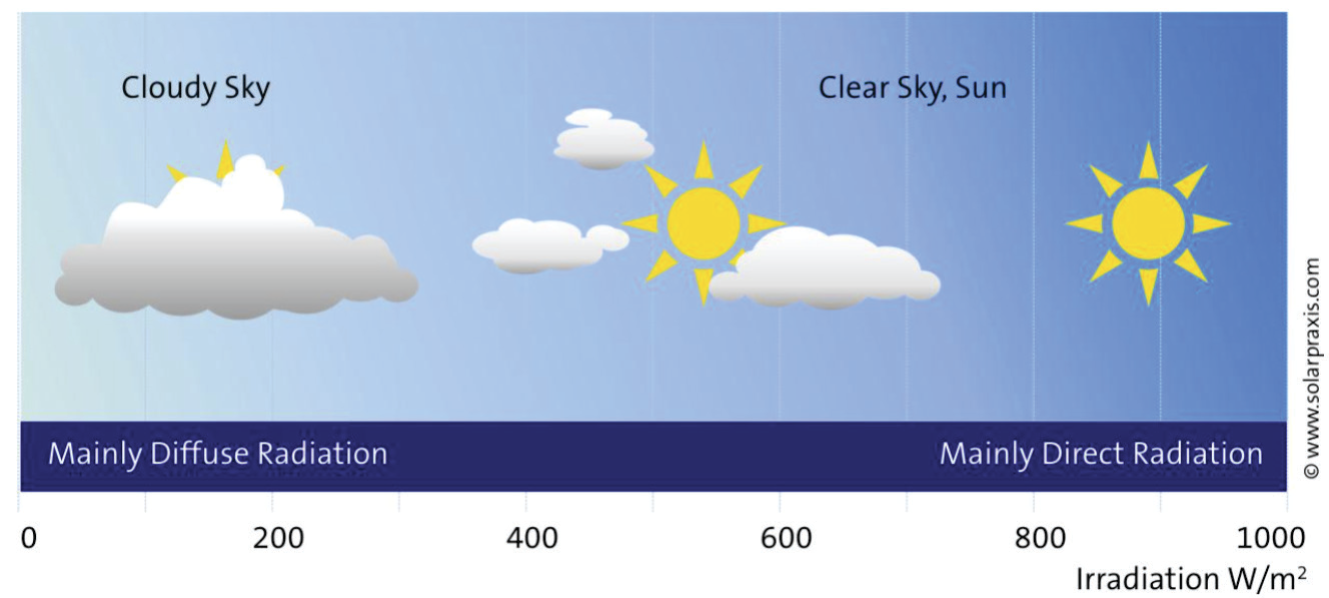
\includegraphics[width=0.65\columnwidth]{images/V01_03.png}



























